\section{Our Implementation}
We constructed  a simple program, which would create a TNFA using the methods description in section~\ref{sec:tnfa} and use it to search data files for matches for a given pattern.

Our implementation supports a series of regular expression symbols, including $+, ^*, |, ?$ along with concatenation of characters. This allows for construction of simple TNFAs from regular expressions, for example the regular expression "(GAT)+" would produce a structure as shown in figure~\ref{fig:gat}

\begin{figure}[h!]
\centering
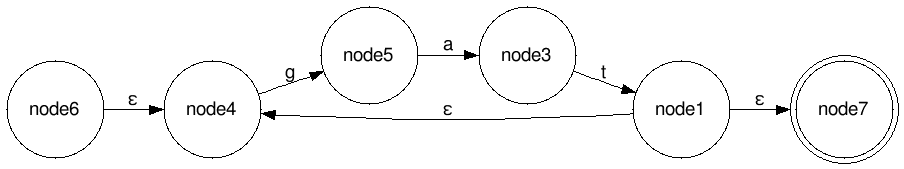
\includegraphics[width=0.5\textwidth]{lib/gat.png}
\caption{Example of how our implementation builds TNFA from regular expression (GAT)+}
\label{fig:gat}
\end{figure}

Each node in the figure has a number corresponding to the time it was created in the code, examining figure~\ref{fig:gat} we can see that the part having GAT was constructed first, and then the surrounding nodes responsible for the $+$ were added onto that, much like one would expect from the description in section~\ref{sec:tnfa}.

When there's a TNFA, our implementation will try each possible transition when matching, causing new states to be made every time two or more possible transitions are viable. For example if there's two epsilon transitions, as in node1 in figure~\ref{fig:gat}, one state will move to node7 and terminate, and another to node4 and continue to match input until it either matches the pattern or is terminated.

If a state can not match a character directly, but it has available insertions, mutations or deletions, it will, for each allowed mismatch,  create a new state, and move accordingly in the TNFA. This way we can guarantee that we will find every possible match for a given pattern. However it also causes an increased runtime given an increase in mismatches, causing one state to spawn up to three new states, and in worst case cause an exponential increase of states until the number of mismatches is exhausted, at which point the states will either match the pattern or be terminated.

%One option for optimization could be to make the transition from tNFA to a deterministic finite automaton or DFA, which we will not describe in detail here. But as a counter argument to this, our implementation was made to primarily focus on matching straightforward RNA sequences with insertions, mutations and deletions, which would result in simple linear NFA's, with little to no epsilon transitions. 